\subsection{Read-your-Writes Consistency}\label{ryw:read-your-writes-consistency}

\subsubsection{Definition}\label{ryw:definition}

Read-your-writes (RYW) consistency guarantees that once a client's write has completed, all subsequent reads by that client observe that write or a later version. Namely, suppose a client writes \emph{x=i} and the write completes successfully. If the same client subsequently reads \emph{x} and obtains \emph{i}, then read-your-writes consistency is preserved. In contrast, if the read returns no value because it reaches a replica that has not yet received the write, the client cannot observe its own completed write, constituting an RYW violation.

\subsubsection{Experimental Design}\label{ryw:experimental-design}

This section aims to investigate how Cassandra handles read-your-writes consistency under different combinations of write and read consistency levels denoted as \emph{W} and \emph{R}, respectively. For each iteration, the script generates a new key and performs one write followed immediately by one read from the same client. The write and read are deliberately sent through different coordinator nodes: by default, the client writes through cass1 and subsequently reads the same key through cass2. This avoids trivially reading the newly written value from the same coordinator and represents situations in which a client reconnects to another node, is redirected by a balancer, or experience driver failover.

For iteration \emph{i}, the client first writes \emph{value=i} to a fresh key using the specified write consistency level \emph{W,} including ONE, QUORUM, and ALL. Once the write has completed successfully, the client immediately reads the same key through the designated read coordinator using consistency level \emph{R}. It is worth noting the architecture of our cluster indicates no artificial waiting period introduced between the two operations but communication between nodes. Then, the outcome of each iteration is classified as a preservation of RYW when \emph{R(x)=i} or a violation against RYW when \emph{R(x)≠i}.

In particular, we use a fresh key in every iteration, making the violation criterion unambiguous. When the write has been confirmed but has not yet become visible to the replicas serving the subsequent read, the read returns None, which will be recorded as a violation. Meanwhile, such implementation also enables us to record a less common case in which a non-null value different from \emph{i} is observed.

\begin{figure}[H]
\centering
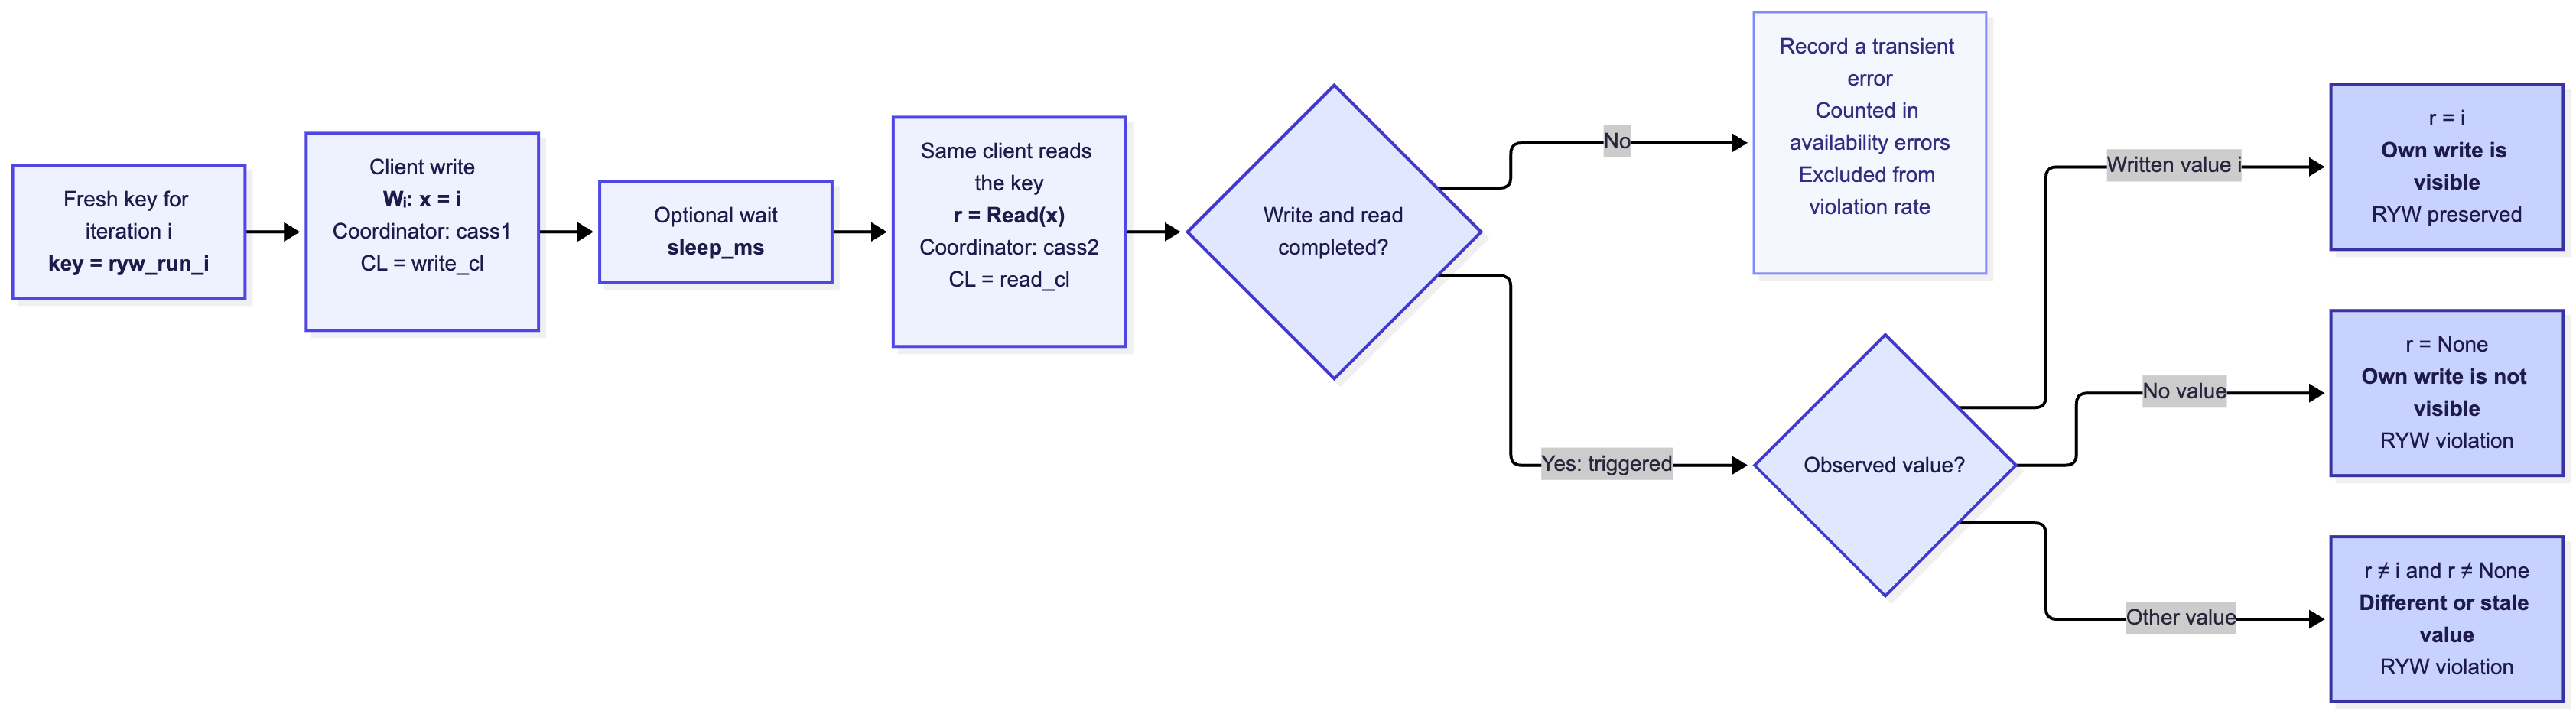
\includegraphics[width=\linewidth]{figures/ryw_flow.png}
\caption{Read-your-writes experimental workflow.}
\label{fig:ryw-flow}
\end{figure}

We will detail the combinations of Cassandra consistency levels in the following:

{
\begin{table}[H]
\centering
\small
\renewcommand{\arraystretch}{1.15}
\caption{RYW consistency-level combinations and replica-set intersection conditions (RF=3).}\label{tab:ryw-1}
\begin{tabular}{@{}lll@{}}
\toprule\noalign{}
Write CL & Read CL & Quorum Relationship (RF=3) \\
\midrule\noalign{}
ONE & ONE & 1+1≤3 \\
ONE & QUORUM & 1+2=3 \\
QUORUM & QUORUM & 2+2\textgreater3 \\
ALL & ONE & 3+1\textgreater3 \\
\bottomrule
\end{tabular}
\end{table}
}

For each configuration above, the test is repeated for the specified number of iterations, and the RYW violation rate is calculated over successfully completed write-read trials. Cassandra timeout or availability exceptions are recorded separately as errors rather than being counted as consistency violations. Each trial additionally records the write and read coordinators, the generated key, written and observed values, and the write timestamp, allowing individual violations to be inspected afterwards.

One last significant component is the injected latency, as we hope to examine how the RYW violation rate changes as the replication window increases. Particularly, we expect weaker consistency-level combinations, like (ONE, ONE) to be more susceptible to violations than the stronger ones.

\subsubsection{Principle and Key Implementation}\label{ryw:principle-and-key-implementation}

The implementation tests visibility after an acknowledged write, rather than the order of competing overwrites. For each fresh key $k_i$, the client waits for the write of value $i$ to complete before issuing the read. In the delay sweep, no additional client-side sleep is inserted. The predicate is $r_i\ne i$, where $r_i$ is the returned value and an absent row is represented by \texttt{None}. Because there is no intentional competing write to the key, equality with $i$ is sufficient for the successful outcome in this workload.

Coordinator selection is controlled through the node-pinned sessions described in Section~\ref{introduction:system-configuration}. Changing the coordinator does not force a particular replica to answer: the read coordinator still selects replicas according to Cassandra's read path. The injected delay targets internode traffic on port 7000, not client CQL traffic on port 9042. This separates the manipulated internode delay from an artificial wait between the client's write and read, although internode read exchanges are also affected.

Let $N=3$ be the replication factor, and let $W$ and $R$ denote the required numbers of write acknowledgements and read responses. For a successful write followed by a successful read of this fresh key, $W+R>N$ forces the read response set to intersect the write acknowledgement set. This supports the expected visibility of the written value for QUORUM/QUORUM and ALL/ONE in this workload. When $W+R\leq N$, intersection is not guaranteed; this permits stale reads but does not determine their frequency. It is not a general proof of all client-centric consistency properties.

Only trials in which both operations complete enter the RYW violation-rate denominator. Timeout and availability exceptions are logged separately, so a failed operation is not classified as either a preserved or a violated read. The reported percentage is
\begin{equation}
\text{RYW violation rate (\%)} =
100\,\frac{\#\{\text{completed trials with }r_i\ne i\}}
{\#\{\text{completed write--read trials}\}}.
\end{equation}
If no trial completes, the rate is undefined rather than zero. The per-iteration trace records the written and observed values, coordinator identities, and any operation error, supporting inspection of individual outcomes.

\subsubsection{Predicted Outcomes}\label{ryw:predicted-outcomes}

Now, we may infer potential outcomes based on the Cassandra read/write consistency levels with corresponding quorum relationship, replication factor, and injected latency. For (ONE, ONE) configuration, we expect it to generate the highest violation rate. In our setup, writes are coordinated by cass1 by default, whereas subsequent reads are coordinated by cass2. Then, such design enables the subsequent read to be served before the newly written value has been copied to the replica. Meanwhile, increasing inter-replica latency may enlarge the window in which an RYW violation can be observed.

For (ONE, QUORUM), we expect violations to remain nontrivial because the exact quorum relationship implied here, 1+2=3=RF, creates a boundary case in which the write and the read replica sets are not guaranteed to overlap. However, requiring a quorum of two replicas for each read increases the likelihood that at least one responding replica has received the latest write, including the write coordinator that holds a local replica. We therefore expect a lower violation rate than under (ONE, ONE), although the rate may still increase with replication latency as the window widens.

For (QUORUM, QUORUM), given that the quorum relationship implies an overlap between the write and read replica sets, a subsequent read following a successful write must include at least one replica that has received the latest write. Cassandra can then reconcile the returned versions based on their timestamps and select the latest value. Therefore, we expect RYW violation to be absent, regardless of the latency level. Similar reasoning may apply to (ALL, ONE). With RF=3, a write consistency level of ALL would request all three replicas to acknowledge the write, then any subsequent read must observe the latest written value. The latency level here will be irrelevant to the consistency outcome but completion time.

\subsubsection{Results and Analysis}\label{ryw:results-and-analysis}

\begin{figure}[H]
\centering
\begin{subfigure}{\linewidth}
\centering
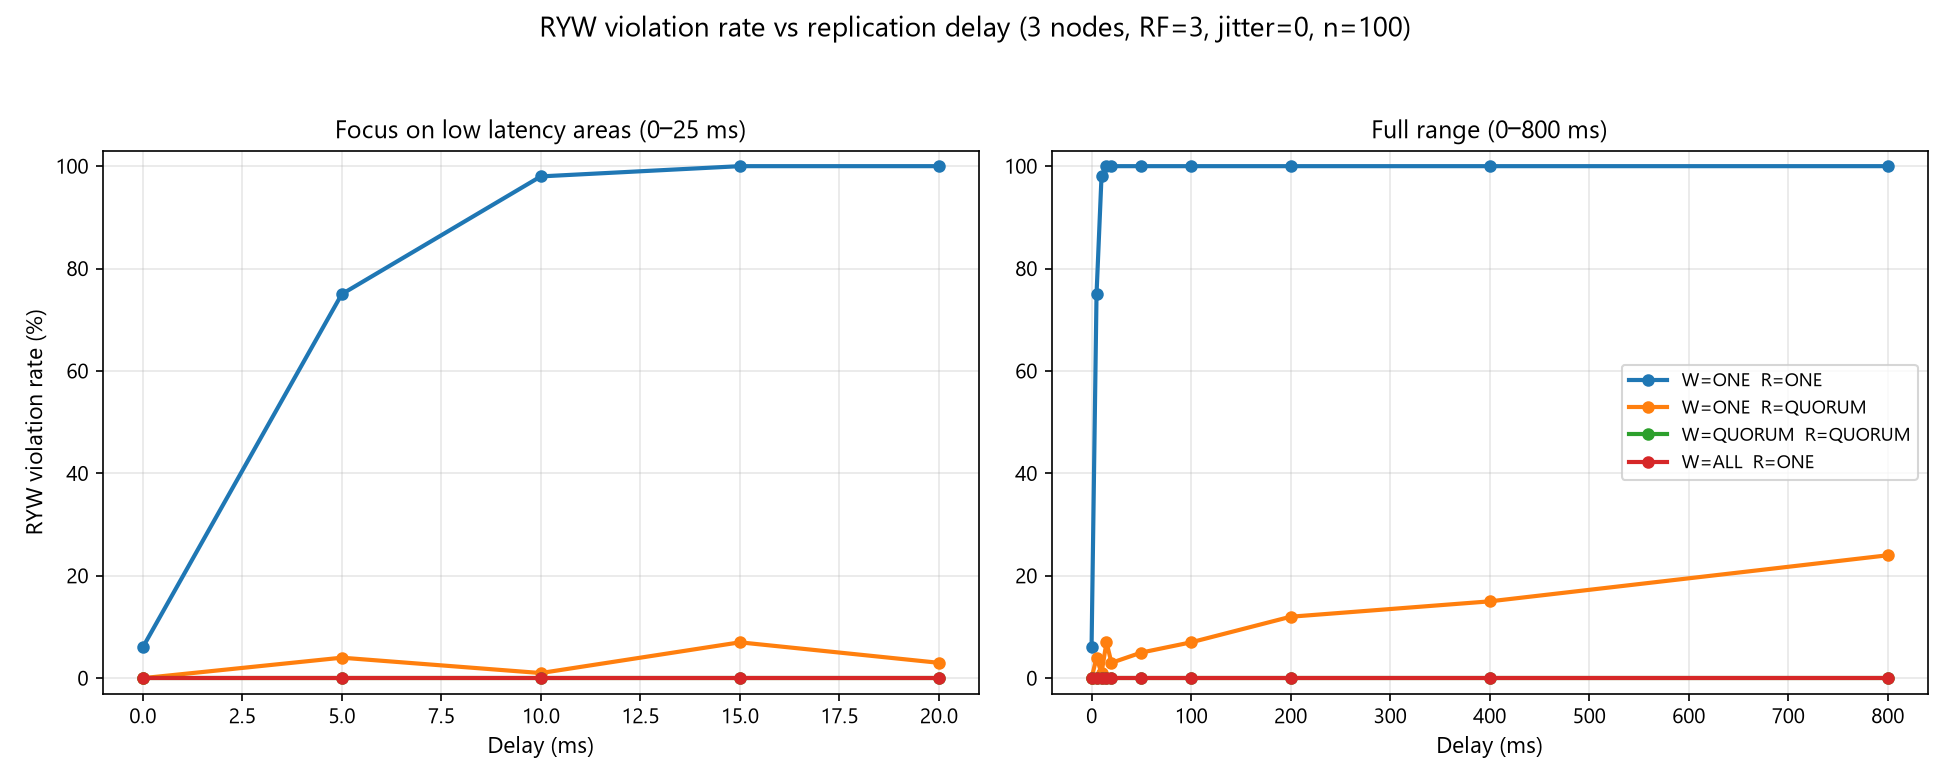
\includegraphics[width=\linewidth]{figures/ryw_macos.png}
\caption{macOS}
\end{subfigure}
\par\medskip
\begin{subfigure}{\linewidth}
\centering
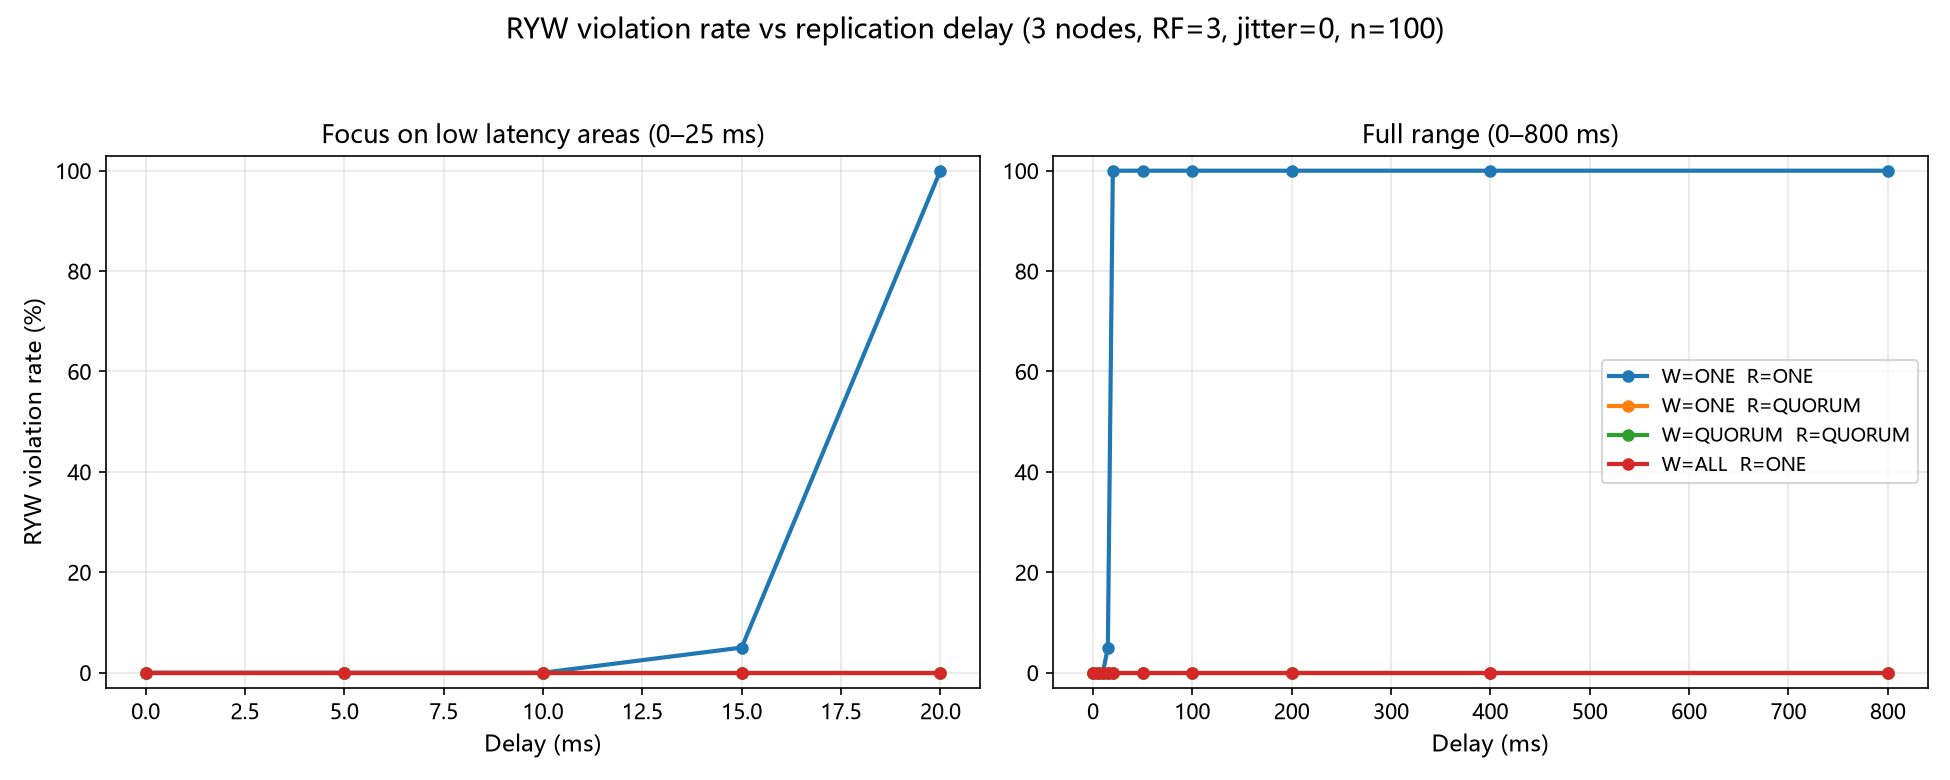
\includegraphics[width=\linewidth]{figures/ryw_windows.png}
\caption{Windows}
\end{subfigure}
\par\medskip
\caption{Comparisons between read-your-writes (RYW) consistency behaviours by hosts on macOS and Windows}
\label{fig:ryw-comparison}
\end{figure}

In order to test RYW consistency in a more heterogeneous environment, we ran the same test on both Windows and macOS hosts, hoping to see whether differences in the underlying operating system and Docker execution would introduce observable variance beyond the general behaviours expected from Cassandra itself. Indeed, while two settings gave similar overall patterns across consistency levels, we did find nuances in their measured violation rates and transition points as latency grows. Nevertheless, we will first interpret the general behaviours shown in the following figure before discussing these platform-specific findings.

As suggested by Figure {[}3{]}, the effect of replication latency on RYW consistency depends strongly on the chosen write and read consistency levels. The most observable effect occurs under (ONE,ONE) setting. Without injected delay, the violation rate remains relatively low, and we attribute such effect to the fact that intra-replica communication moves faster than the time lapse between two consecutive write and read requests from the client's end. However, once a small delay is introduced, it rises sharply and further converges to 100\% no later than 20ms. Disregarding jitters and hardware variance, we may interpret this decisive latency level threshold as a rough approximation of the time difference between the point where the replication is finished and accessible to the coordinator and the point when the read request arrives. Beyond this level, we found any further increases in latency produce nearly no additional change, indicating that the violation rate has effectively saturated. This behaviour is actually consistent with the weak overlapping relationship between write and read replica sets of (ONE, ONE), as introducing larger latency will enlarge the window in which a subsequent read may be satisfied before the latest write has propagated successfully.

Another material pattern is observed under (ONE, QUORUM). As expected, violations remain well below those of (ONE, ONE) and still preserve a nearly non-decreasing relationship with latency level. However, at higher latency, the violation rate rises steadily rather than converging sharply. This is also consistent with the boundary quorum relationship, where W+R=1+2=3=RF, under which overlap between the write and read replica sets is possible but not surely guaranteed. Requiring two replica responses nevertheless has a non-trivial probability that the read request is handled by a replica containing the last write. It is further suggesting that the fluctuations in high latency regime can be explained by not only the replica participation of individual requests but the timing, where the latter factor was indeed dominated by the former one.

In contrast, (QUORUM, QUORUM) and (ALL, ONE) gave us no substantial violations throughout the tested latency range. This is again consistent with our inference on quorum relationship and it indicates that the injected latency for replication is now independent of the write/read consistency level but solely of how fast these operations will be completed.

Finally, we can proceed to discuss the cross-platform differences separately as variations in the execution and request-handling schemes rather than as changes to these underlying consistency relationships. We repeated the delay sweep tests on a Windows host and a macOS host (n=100, jitter=0). The two platforms agree on the general pattern, where combinations (QUORUM, QUORUM) and (ALL, ONE) stay at 0\% at every delay, and (ONE, ONE) converges to 100\% in high-latency regime. However, two platforms differ in where the other two configurations rise. On one hand, for (ONE, ONE), macOS is already at 75\% at 5ms whereas Windows shows no violation up to 10ms. On the other, Windows shows no violation at all for (ONE, QUORUM), while macOS shows nearly 8\% at delays of 5ms and above. Yet the absence of violations under (ONE, QUORUM) on Windows is not general because when we later introduced jittered delay, we observed the same host violates in 1.5\% (10ms delay, 10ms jitter), 14.5\% (50ms delay, 50ms jitter) and 19.3\% (100ms, 50ms), a seemingly compound effects from delay-jitter combinations.

To figure out where these cross-platform differences come from, we composed a diagnostic version of the RYW test (experiments/ryw\_diagnostic.py) that runs the same sequence but enables Cassandra query tracing for both requests and stores one JSON record per iteration, including the platform, read/write coordinator, replica addresses, client-end timestamp, etc. By detailing these factors, we are able to answer questions like which replica the read coordinator asked for and when each message left one node and reached the next. Interestingly, it is in these answers that we figured out potential explanations of those differences.

We ran the diagnostic script for (ONE, QUORUM) on both hosts (100ms, n=20). Both runs showed a 1/20 violation rate, and while these numbers are too few to be statistically significant, tracing how they work shows the mechanism. Normally, the read coordinator, cass2, reads its own copy, then asks one other replica for a digest. Asking cass1 always finds the row, yet asking cass3 is a race between the replication and the digest request, and a violation only happens when the digest request wins.

The replication leaves cass1 as soon as the write is processed, while the digest request only leaves cass2 after the client's write is acknowledged. Because that write call took much longer on Windows (13.8ms median vs.~4ms on macOS), the digest request also starts later on Windows, giving the replication roughly 10ms more time to arrive first. This is also consistent with the observation we had on (ONE, ONE), where the violation rate only starts to rise when the injected latency is larger than 10ms.

Additionally, we may bring up another minor yet inspiring finding that the two hosts don't pick the same replica as often. Out of our 20 reads in our diagnostic test, cass2 asked cass1 for a digest 15 times on Windows but only 7 times on macOS, nudging Windows toward fewer violations. This choice is made by Cassandra's dynamic snitch based on observed replica latency, rather than directly by the client. However, with only 20 samples per run, we cannot rule out sampling noise as an explanation for the observed split.

\subsubsection{Limitations}\label{ryw:limitations}

These results are specific to our three-container setup and the tested request paths. Pinning a coordinator does not fix which replicas answer a read, and the delay applied to port 7000 affects internode read traffic as well as write propagation. We disabled read repair and speculative retry to make the behavior easier to observe, so the measured rates should not be treated as rates for Cassandra's default configuration. Each delay point contains 100 trials, while the tracing comparison contains only 20 per host; we did not calculate confidence intervals. Tracing also adds overhead. Thus, the two hosts' different rates and timings suggest possible mechanisms, but do not establish an operating-system effect.